\section{Durchführung und Aufbau}
\label{Aufbau}
\subsection{Aufbau}
In Abbildung (\ref{fig:aufbau1}) ist die Messapparatur graphisch dargestellt.
\begin{figure}
	\centering
	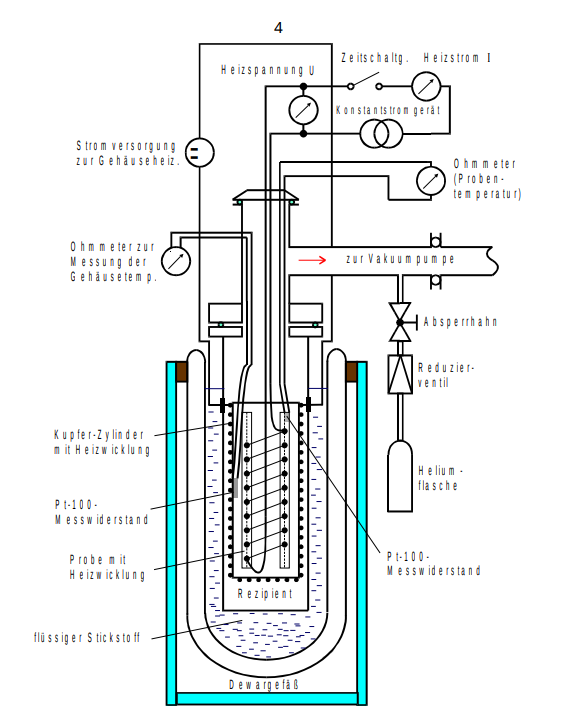
\includegraphics[scale=0.5]{fig/aufbau.png}
	\caption{Schematischer Aufbau der Messapparatur \cite[4]{Anleitung}.}
	\label{fig:aufbau1}
\end{figure}
\FloatBarrier
\noindent Die Kupferprobe, die untersucht wird, befindet sich innerhalb eines Zylinders im Rezipienten und ist zur Wärmeisolation von einem Dewar-Gefäß umhüllt.
Für die Messung der Temperatur von Zylinder und Probe sind zwei Pt-100-Widerstände vorhanden. Desweiteren werden noch Heizwicklungen zur Regulierung der Temperatur von Probe und Zylinder benötigt.
\subsection{Durchführung}
Am Anfang des Versuches wird der Rezipient mithilfe der Vakuumpumpe evakuiert. Im Anschluss daran wird dieser dann mit Helium befüllt um einen guten Wärmeaustausch zwischen Zylinder und Probe zu
Gewährleisten. Durch Einfüllen von flüssigem Stickstoff in das Dewar-Gefäß soll die Probe nun auf $T=\SI{80}{\kelvin}$ abgekühlt werden. Ist die Temperatur erreicht wird nun erneut evakuiert und die
eigentliche Messung kann beginnen. Dabei werden die Kupferprobe als auch der Zylinder um diese kontinuierlich erhitzt. In Abständen von etwa $\SI{10}{\kelvin}$ werden nun Messdaten für
Stromstärke $I$, Spannung $U$, die beiden Widerstandswerte $R_\mathrm{i}$ sowie die benötigte Zeit $\Delta t$, aufgenommen. Wenn die Probe Raumtemperatur erreicht, ist die Messung abgeschlossen.
